\documentclass[10pt]{article}
\usepackage{stdstyle}


\title{Coherent Interactions in a Three-Level System}
\author{Yi Zhu}
\date{December 7, 2025\footnote{Updated \today}}

\begin{document}

\maketitle

\section{Hamiltonian}

\begin{figure}[H]
    \centering
    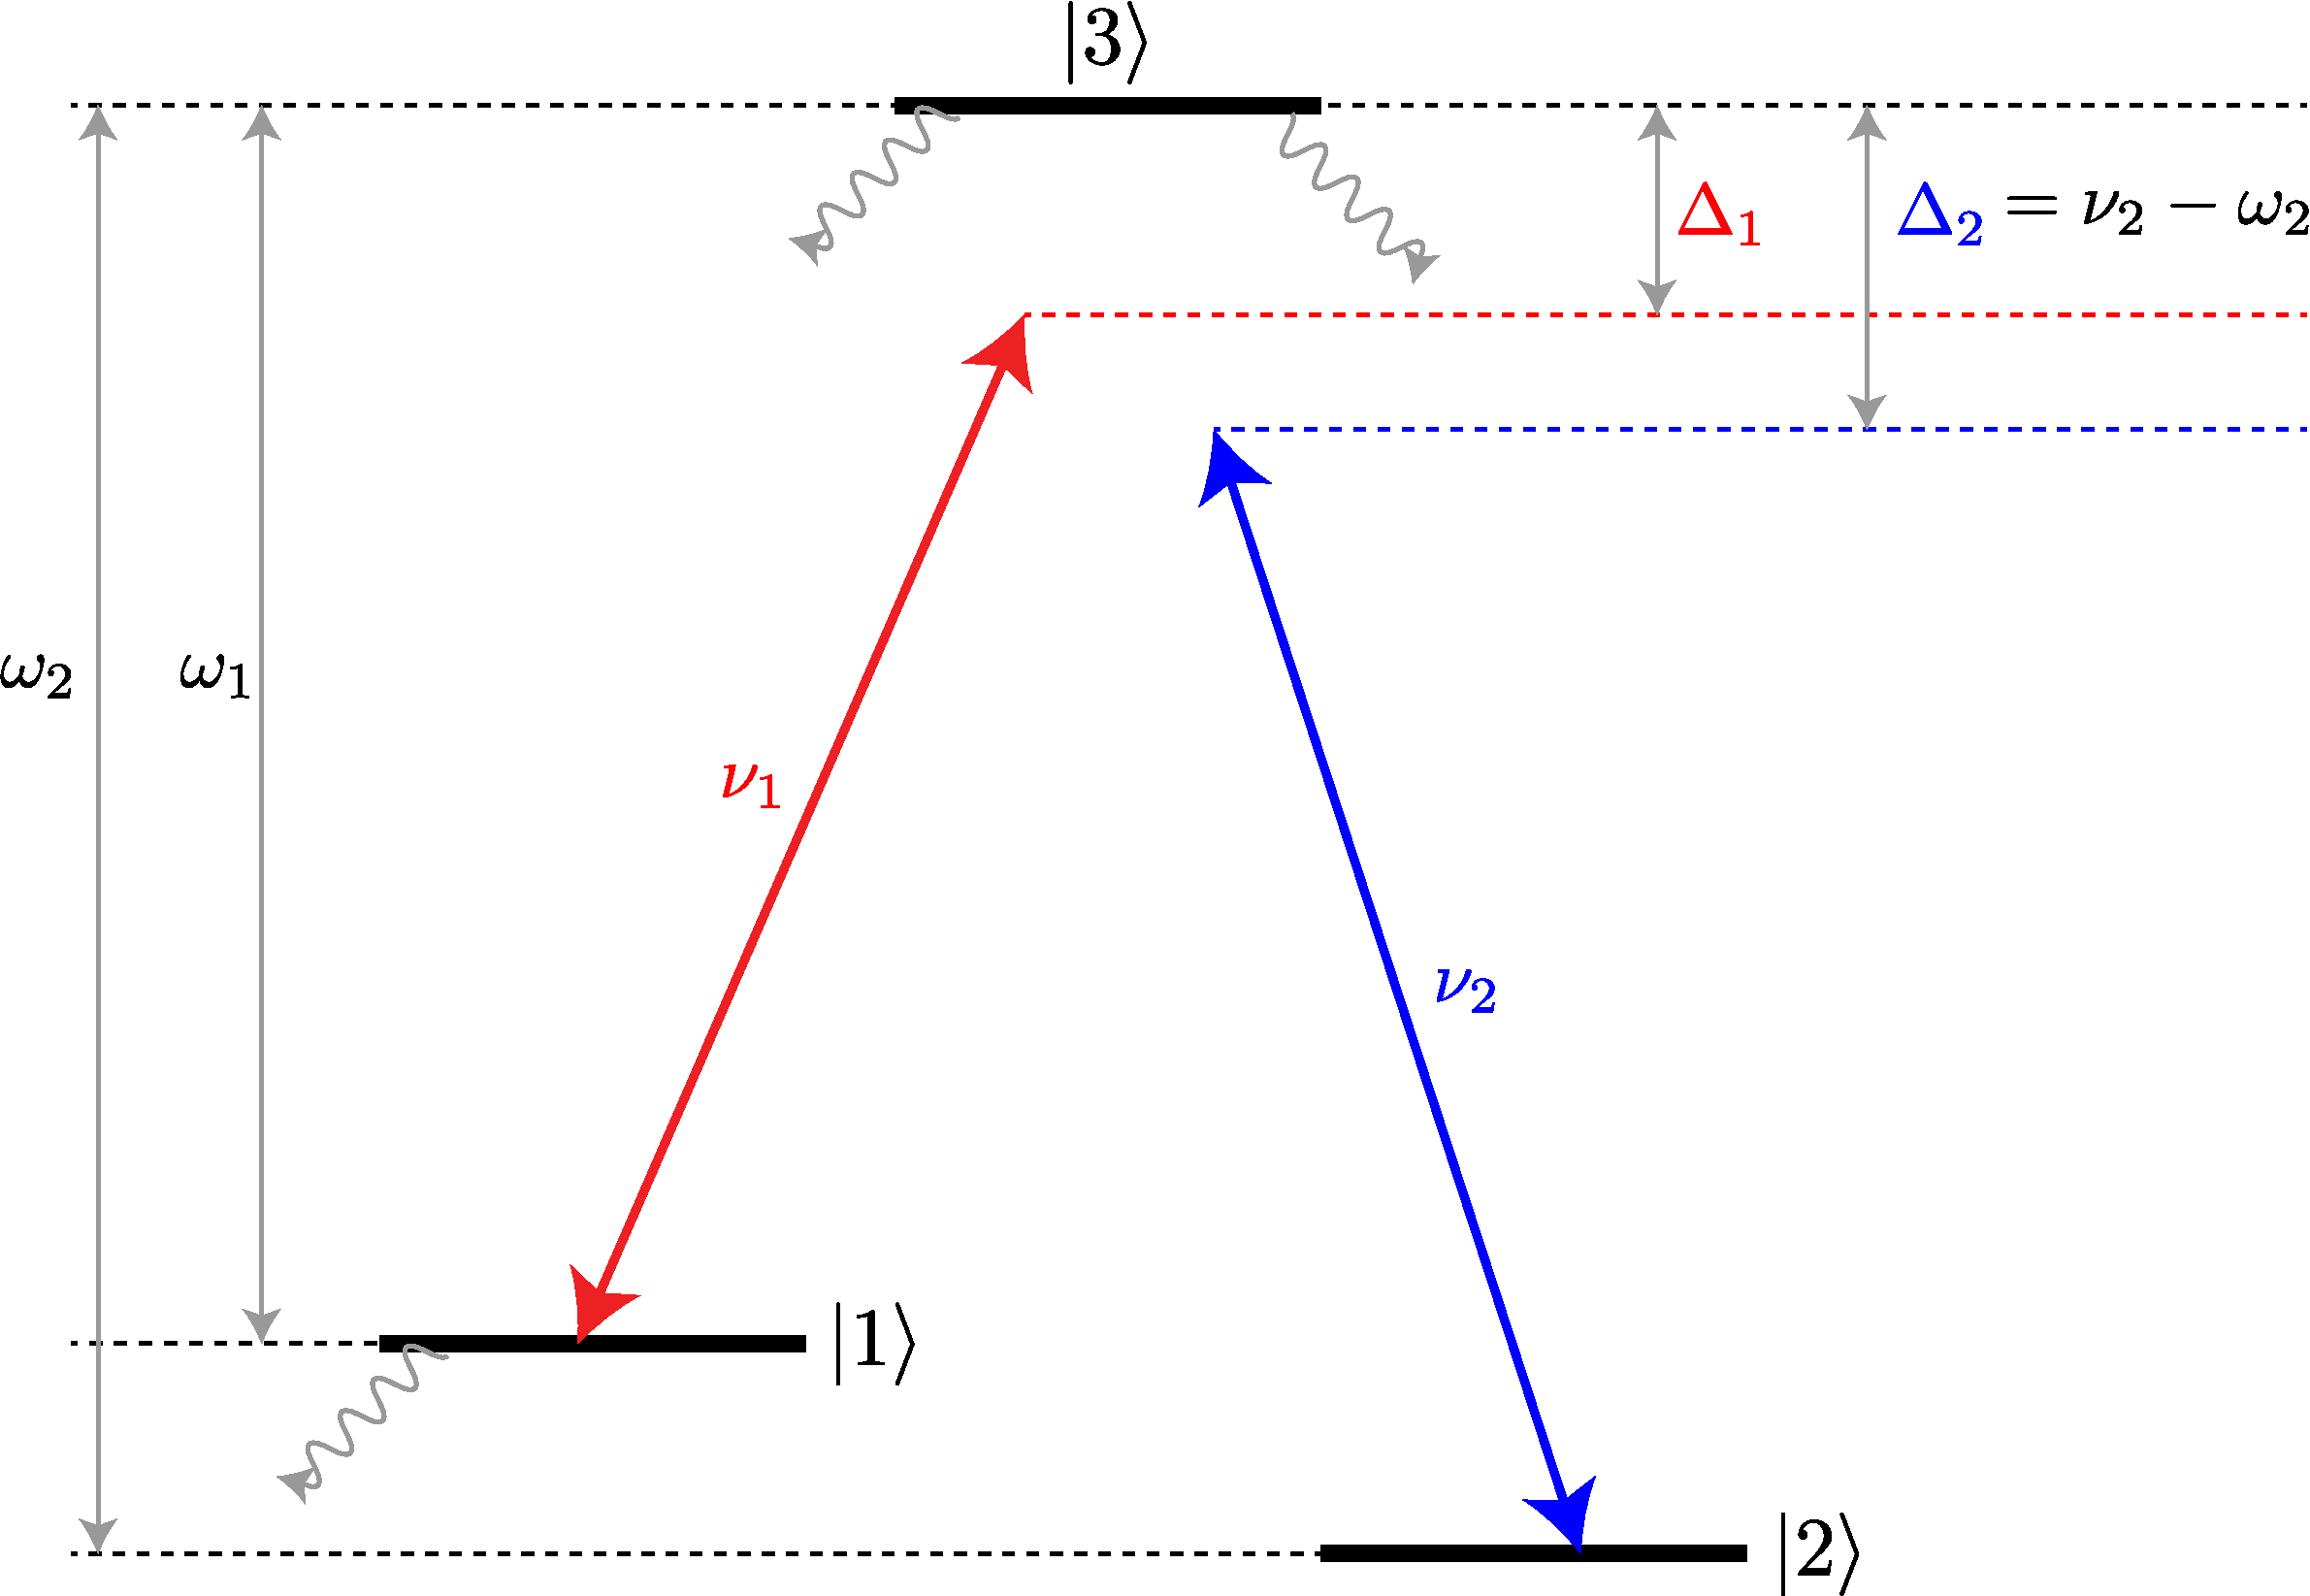
\includegraphics[width=0.6\linewidth]{fig/Raman.pdf}
    \caption{Three-level system. We define $\ket{3}$ to be the zero-energy point and assume $\ket{2}$ is the ground state.}
    \label{fig:raman}
\end{figure}
The Hamiltonian for (fig. \ref{fig:raman}) is,
\begin{equation}
    H = -\hbar\omega_1\ketbra{1}{1} -\hbar\omega_2\ketbra{2}{2} - \boldsymbol{d}\cdot\mathbf{E}\quad\text{where}\quad \mathbf{E}(t) = \boldsymbol{\varepsilon_1} e^{-i\nu_1t} + \boldsymbol{\varepsilon_2} e^{-i(\nu_2t + \phi)} + \text{h.c.}
\end{equation}
and $\phi$ is the phase difference between the two lasers. For $\mu_{ij} = \mel{i}{\hat{d}}{j}$ real,
\begin{align}
    H = -\hbar\omega_1\ketbra{1}{1} -\hbar\omega_2\ketbra{2}{2} &- \mu_{13}( \ketbra{1}{3} + \ketbra{3}{1} )(\varepsilon_1 e^{-i\nu_1 t} + \varepsilon_1^* e^{i\nu_1 t}) \nonumber\\
    &- \mu_{23} ( \ketbra{2}{3} + \ketbra{3}{2} )(\varepsilon_2 e^{-i(\nu_2 t+\phi)} + \varepsilon_2^* e^{i(\nu_2 t+\phi)})
\end{align}

\section{Moving to Rotating Frame}

Now we move into the rotating frame via the unitary,
\begin{equation}
    U = e^{-i\nu_1 t}\ketbra{1}{1} + e^{-i\nu_2 t}\ketbra{2}{2} + \ketbra{3}{3}
\end{equation}
In other words, in the rotating frame, the state, Hamiltonian, and a general operator $O$ respectively become,
\begin{align}
    \ket{\psi} &\rightarrow U\ket{\psi}\\
    H &\rightarrow UHU^\dagger + i\hbar\dot{U}U^\dagger\\
    O &\rightarrow UOU^\dagger
\end{align}
Therefore the Hamiltonian in the rotating frame becomes,
\begin{align}
    H &= 
    \begin{pmatrix}
        -\hbar\omega_1 & 0 & \mu_{13}(\varepsilon_1^* + \varepsilon_1e^{-2i\nu_1 t}) \\
        0 & -\hbar \omega_2 & \mu_{23}(e^{i\phi}\varepsilon_2^* + e^{-i\phi}\varepsilon_2e^{-2i\nu_2 t}) \\
        \mu_{13}(\varepsilon_1 + \varepsilon_1^* e^{2i\nu_1 t}) & \mu_{23}(e^{-i\phi}\varepsilon_2 + e^{i\phi}\varepsilon_2^* e^{2i\nu_2 t}) & 0
    \end{pmatrix}
    +
    \begin{pmatrix}
        \hbar\nu_1 & 0 & 0\\
        0 & \hbar \nu_2 & 0 \\
        0 & 0 & 0
    \end{pmatrix}
    \\
    &=
    \begin{pmatrix}
        -\hbar(\omega_1-\nu_1) & 0 & \mu_{13}(\varepsilon_1^* + \varepsilon_1e^{-2i\nu_1 t}) \\
        0 & -\hbar (\omega_2 -\nu_2) & \mu_{23}(e^{i\phi}\varepsilon_2^* + e^{-i\phi}\varepsilon_2e^{-2i\nu_2 t}) \\
        \mu_{13}(\varepsilon_1 + \varepsilon_1^* e^{2i\nu_1 t}) & \mu_{23}(e^{-i\phi}\varepsilon_2 + e^{i\phi}\varepsilon_2^* e^{2i\nu_2 t}) & 0
    \end{pmatrix}
\end{align}
Note that we often denote the rotating frame Hamiltonian as $\Tilde{H}$, but it has been omitted here to avoid notational clutter. We are laissez-faire about notating the rotating frame, because observables are not affected by frame transformations (see below). However, keep in mind that the operators in rotating frame are not the same operators in the lab frame. For example, $\Tilde{\sigma}_x$ in the rotating frame (but we drop the tilde and write as $\sigma_x$) is not the same operator as $\sigma_x$ (in the lab frame).
\begin{equation}
    \langle\Tilde{\psi} | \Tilde{O} | \Tilde{\psi} \rangle = \bra{\psi}U^\dagger \, (UOU^\dagger) \, U\ket{\psi} = \mel{\psi}{O}{\psi}
\end{equation}
Now, define the following quantities,
\begin{equation}
    \text{detuning: }\Delta_i = \omega_i-\nu_i\quad\text{and}\quad\text{Rabi frequency: }\Omega_i=\varepsilon_i\mu_{i3}/\hbar
\end{equation}
Then we can rewrite the Hamiltonian as,
\begin{equation}
    H = -\hbar\Delta_1\ketbra{1}{1} -\hbar\Delta_2\ketbra{2}{2} - \hbar\left[(\Omega_1^* + \Omega_1 e^{-2i\nu_1 t})\ketbra{1}{3} + (e^{i\phi}\Omega_2^* + e^{-i\phi}\Omega_2e^{-2i\nu_2 t}) \ketbra{2}{3} + \text{h.c.} \right]
    \label{eq:H_full}
\end{equation}

\section{Rotating Wave Approximation}

We use the rotating wave approximation (RWA) to eliminate the time-dependent terms in (eq. \ref{eq:H_full}) under appropriate conditions. Before discussing the RWA in detail, note that in the original definition of the Hamiltonian we have assumed a classical electromagnetic field. If instead we quantized the electromagnetic field (i.e. in the case of Jaynes-Cummings Hamiltonian), then a laser with frequency $\nu$ would correspond to,
\begin{equation}
    \boldsymbol{E}(t) = \hat{a}\,\boldsymbol{\varepsilon}e^{-i\nu t} + \hat{a}^\dagger\,\boldsymbol{\varepsilon}^*e^{i\nu t}
\end{equation}
Therefore, the time-independent terms in the Hamiltonian (eq. \ref{eq:H_full}) correspond to operators like,
\begin{equation}
    \ketbra{1}{3}\hat{a}^\dagger\quad \text{and}\quad\ketbra{3}{1}\hat{a}
\end{equation}
which are energy conserving; while time-dependent terms correspond to operators like,
\begin{equation}
    \ketbra{1}{3}\hat{a} \quad \text{and} \quad \ketbra{3}{1}\hat{a}^\dagger
\end{equation}
which are \textit{not} energy conserving. These terms in the Hamiltonian are also called the \textit{counter-rotating} terms. Processes corresponding to these terms are ``virtual'' --- consistent with the quickly oscillating phase of these operators (in the analogy of virtual particles, these processes must be quick to satisfy energy-time uncertainty). We can eliminate these terms if the following the driving fields are weak: $\Omega_i\ll\nu_i$. To derive this condition, let's treat the counter-rotating terms perturbatively.
\begin{align}
    H &= H_0 + (\hbar\Omega_1 e^{-2i\nu_1t}\ketbra{1}{3} + \hbar\Omega_2 e^{-2i\nu_2t}\ketbra{2}{3} + \text{h.c.}) \\
    &= H_0 + H'(t)
\end{align}
Then the first-order correction from time-dependent perturbation theory is,
\begin{equation}
    |\psi^{(1)}(t)\rangle = \int_0^t H'(t')\ket{\psi(0)}\,\dd t'
\end{equation}
Which results in terms with magnitude bounded by (in units of $\hbar=1$),
\begin{equation}
    \abs{\int_0^t \Omega_i e^{\pm 2i\nu_i t'}\dd t'} = \abs{\Omega\frac{e^{\pm 2i\nu_i t}-1}{\pm 2i\nu_i t}} = \frac{\Omega}{\nu}
\end{equation}

\begin{figure}[H]
    \centering
    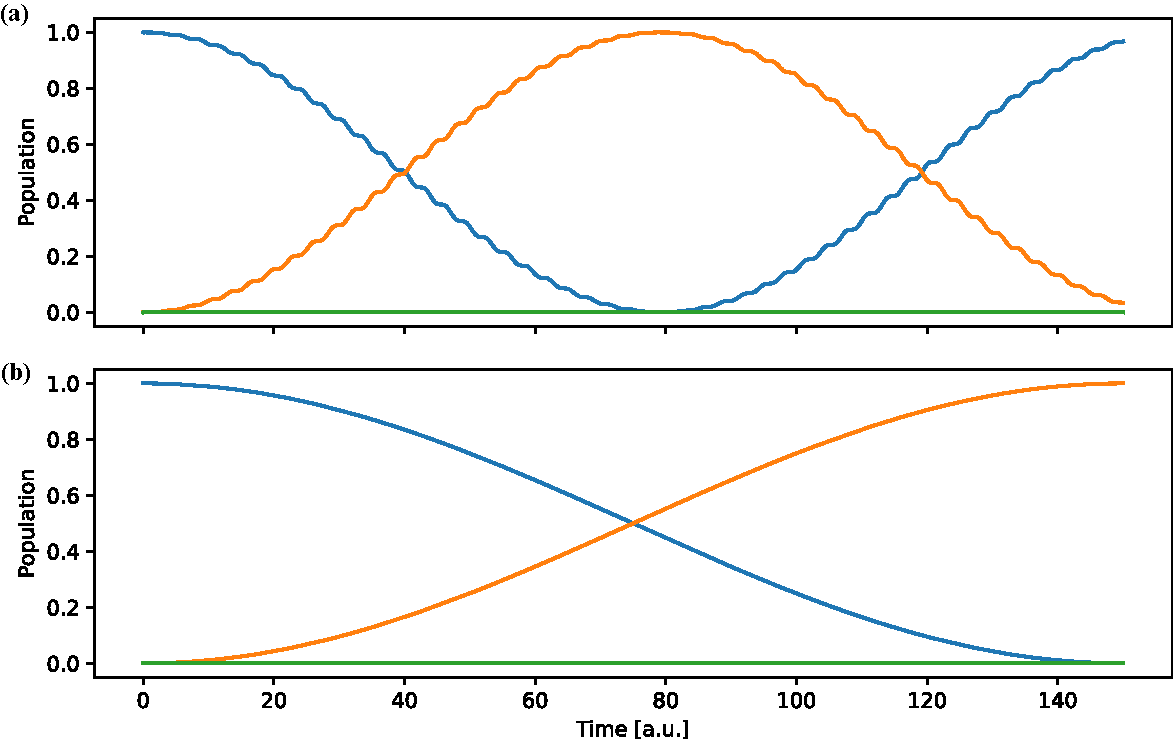
\includegraphics[width=0.7\linewidth]{fig/rwa.pdf}
    \caption{Numerical evolution of (eq. \ref{eq:H_full}) for $\Omega_i=1$, $\Delta_i=100$, and $\phi=0$. Blue: population in $\ket{1}$; orange: in $\ket{2}$; and green in $\ket{3}$. \textbf{(a)} with $\nu_i=1$. \textbf{(b)} with $\nu_i=1000$. Despite constant $\Omega_i,\Delta_i$, the effective Rabi frequency increases by a factor of 2 when moving out of the RWA regime (when $\nu_i$ becomes similar/smaller than other timescales). This is because in the limit $\nu_i=0$, $e^{-2i\nu_i t}=1$ so $\Omega_i$ is effectively doubled in (eq. \ref{eq:H_full}) whereas in the RWA treatment $e^{-2i\nu_i t}$ averages to zero.}
    \label{fig:rwa}
\end{figure}
With the RWA, the Hamiltonian becomes,
\begin{equation}
    H = -\hbar\Delta_1\ketbra{1}{1} -\hbar\Delta_2\ketbra{2}{2} - \hbar\left(\Omega_1^* \ketbra{1}{3} + e^{i\phi}\Omega_2^* \ketbra{2}{3} + \text{h.c.} \right)
    \label{eq:RWA}
\end{equation}

\section{Adiabatic Elimination}

For notational convenience, let $\Delta = \Delta_2$ and define the \textit{two-photon detuning} $\delta=\Delta_1-\Delta_2$. Then we can represent (eq. \ref{eq:RWA}) as,
\begin{equation}
    H = -\hbar
    \begin{pmatrix}
        \Delta_1 & 0 & \Omega_1^*\\
        0 & \Delta_2 & e^{i\phi}\Omega_2^*\\
         \Omega_1& e^{-i\phi}\Omega_2 & 0
    \end{pmatrix}
    =
    -\hbar
    \begin{pmatrix}
        \delta & 0 & \Omega_1^*\\
        0 & 0 & e^{i\phi}\Omega_2^*\\
         \Omega_1& e^{-i\phi}\Omega_2 & -\Delta
    \end{pmatrix}
\end{equation}
With $\ket{\psi} = c_1(t)\ket{1} + c_2(t)\ket{2} + c_3(t)\ket{3}$, we can write the Schroedinger equation as,
\begin{align}
    \dot{c}_1(t) &= i\delta\,c_1(t) + i\Omega_1^*\,c_3(t) \\
    \dot{c}_2(t) &= ie^{i\phi}\Omega_2^*\,c_3(t)\\
    \dot{c}_3(t) &= i\Omega_1\,c_1(t) + ie^{-i\phi}\Omega_2\,c_2(t) - i\Delta\,c_3(t) \label{eq:c3}
\end{align}
We often want to consider the case where $\Delta$ is far detuned (and the two-photon detuning is small). In this case, notice that $i\Delta\,c_3(t)$ is much larger than the remaining terms in the differential equations for $c_i(t)$. Let's examine (eq. \ref{eq:c3}) in greater detail. First rearrange then multiply both sides of the equation by $e^{i\Delta}t$,
\begin{align}
    e^{i\Delta t}(i\Omega_1\,c_1(t) + ie^{-i\phi}\Omega_2\,c_2(t)) &= e^{i\Delta t}(\dot{c}_3(t) + i\Delta\,c_3(t)) \\
    &=\frac{\dd}{\dd t}\left( e^{i\Delta t}\,c_3(t) \right) \\
    \int_0^t e^{i\Delta t'}\left[ i\Omega_1\,c_1(t') + ie^{-i\phi}\Omega_2\,c_2(t')\right]\,\dd t' &= e^{i\Delta t}\,c_3(t) - c_3(0)
\end{align}
With $c_3(0) = 0$,
\begin{equation}
    c_3(t) = e^{-i\Delta t} \int_0^t e^{i\Delta t'}\left[ i\Omega_1\,c_1(t') + ie^{-i\phi}\Omega_2\,c_2(t')\right]\,\dd t'
\end{equation}
The term in the integral is rapidly oscillating which averages to zero after a cycle of oscillation. Only during the small duration $\sim1/\Delta$ near the upper integrand $t'=t$ do the terms in the integral not cancel. But again, since $\Omega\ll\Delta$, this contribution is effectively constant. Therefore, $c_3(t)$ is effectively constant and the result of the \textit{adiabatic elimination} is that $\dot{c}_3(t) = 0$. Which implies that $c_3(t)$ directly follows the population in $c_1(t)$ and $c_2(t)$.
\begin{equation}
    0 = i\Omega_1\,c_1(t) + ie^{-i\phi}\Omega_2\,c_2(t) - i\Delta\,c_3(t)
\end{equation}
\begin{equation}
    c_3(t) = \frac{\Omega_1\,c_1(t) + e^{-i\phi}\Omega_2\,c_2(t)}{\Delta}
\end{equation}
Plugging in this approximation for $c_3(t)$,
\begin{align}
    \dot{c}_1(t) &= i\left(\delta + \frac{\abs{\Omega_1}^2}{\Delta}\right)\,c_1(t) + i\left(\frac{e^{-i\phi}\Omega_1^*\Omega_2}{\Delta}\right)\,c_2(t) \\
    \dot{c}_2(t) &= i\left( \frac{e^{i\phi}\Omega_1\Omega_2^*}{\Delta} \right)\,c_1(t) + i\left( \frac{\abs{\Omega_2}^2}{\Delta} \right)\,c_2(t)
\end{align}
This corresponds to the effective two-level Hamiltonian in the $\{\ket{1}, \ket{2}\}$ basis,
\begin{equation}
    H = 
    \hbar
    \begin{pmatrix}
        \delta + \frac{\abs{\Omega_1}^2}{\Delta} & \frac{e^{-i\phi}\Omega_1^*\Omega_2}{\Delta} \\
        \frac{e^{i\phi}\Omega_1\Omega_2^*}{\Delta} & \frac{\abs{\Omega_2}^2}{\Delta}
    \end{pmatrix}
\end{equation}
Taking $\Omega_1$ and $\Omega_2$ to be real,
\begin{equation}
    H =  \hbar\left(\delta + \frac{\Omega_1^2 - \Omega_2^2}{\Delta}\right)\,\sigma_z + \hbar\frac{\Omega_1\Omega_2}{\Delta}\left[\cos(\phi)\,\sigma_x + \sin(\phi)\,\sigma_y\right]
\end{equation}



\end{document}
